% Draft content for the interim report.
% Paste this into the Overleaf template body.

\section{02\_CNN\_Introduction}

\subsection{Task 1: Classification}
\textbf{Report (classification):}
\begin{itemize}
  \item \textbf{Bar figure and discussion.} We compared four CNN designs on CIFAR-10 (Figure~\ref{fig:cnn_bar}). Depth and max pooling gave the largest gains; average pooling underperformed. Training accuracy is consistently higher than validation accuracy, indicating mild overfitting as model capacity increases.
  \item \textbf{Best architecture sketch.} The best design was \texttt{3conv\_32\_64\_128\_max} (Figure~\ref{fig:cnn_arch}).
\end{itemize}

\begin{figure}[!ht]
  \centering
  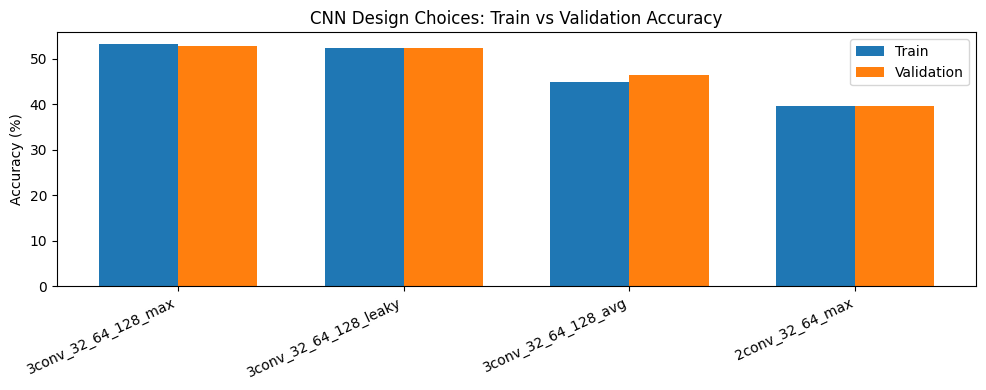
\includegraphics[width=0.9\columnwidth]{figs/cnn_task1_bar.png}
  \caption{Training vs.\ validation accuracy for four CNN design choices (Task 1).}
  \label{fig:cnn_bar}
\end{figure}

\begin{figure}[!ht]
  \centering
  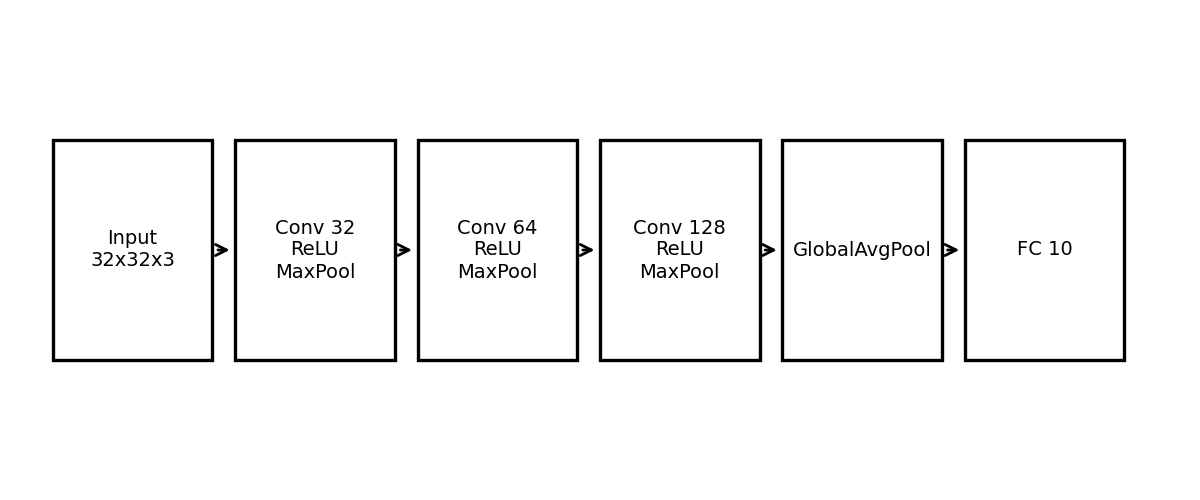
\includegraphics[width=0.75\columnwidth]{figs/cnn_task1_arch.png}
  \caption{Sketch of the best architecture: \texttt{3conv\_32\_64\_128\_max}.}
  \label{fig:cnn_arch}
\end{figure}

\begin{table}[!ht]
  \centering
  \small
  \setlength{\tabcolsep}{4pt}
  \caption{Best training/validation accuracy (\%) per design choice.}
  \label{tab:cnn_task1_acc}
  \begin{tabular}{lcc}
    \toprule
    Design & Train & Val \\
    \midrule
    3conv\_32\_64\_128\_max & 53.15 & 52.72 \\
    3conv\_32\_64\_128\_leaky & 52.35 & 52.36 \\
    3conv\_32\_64\_128\_avg & 44.96 & 46.35 \\
    2conv\_32\_64\_max & 39.65 & 39.51 \\
    \bottomrule
  \end{tabular}
\end{table}

\subsection{Task 2: Regression}
\textbf{Report (regression):}
\begin{itemize}
  \item \textbf{Architecture with validation error $<75\%$.} All three CNN regressors achieved validation MAPE below 75\%, and the widest model performed best (Table~\ref{tab:reg_mape}).
  \item \textbf{Training/validation loss vs.\ epochs.} Loss curves are shown in Figure~\ref{fig:reg_loss}. The wider model reduces validation error but increases the train--val gap later in training.
  \item \textbf{Other house sections.} Results for kitchen, bedroom, and bathroom are reported in Table~\ref{tab:reg_mape}.
\end{itemize}

\begin{figure}[!ht]
  \centering
  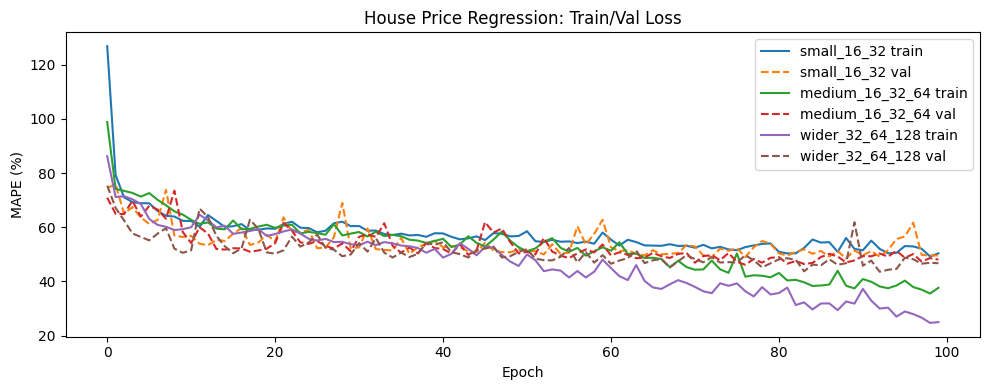
\includegraphics[width=0.9\columnwidth]{figs/cnn_task2_loss.png}
  \caption{Training and validation loss vs.\ epochs for regression architectures.}
  \label{fig:reg_loss}
\end{figure}

\begin{table}[!ht]
  \centering
  \small
  \setlength{\tabcolsep}{4pt}
  \caption{Best validation MAPE (\%) for regression models and room sections.}
  \label{tab:reg_mape}
  \begin{tabular}{l c | l c}
    \toprule
    Architecture & MAPE & Section & MAPE \\
    \midrule
    wider\_32\_64\_128 & 43.59 & frontal & 49.64 \\
    medium\_16\_32\_64 & 46.17 & kitchen & 50.23 \\
    small\_16\_32 & 48.51 & bathroom & 57.25 \\
    \phantom{small} & \phantom{00.00} & bedroom & 59.08 \\
    \bottomrule
  \end{tabular}
\end{table}

\section{03\_Network\_Training}

\subsection{Task 1: Tuning a Classification Model}
\textbf{Report (tuning a classification model):}
\begin{itemize}
  \item \textbf{Data augmentation.} We trained the baseline without augmentation and two strategies: \textbf{Aug1} = RandomCrop(32, padding=4) + RandomHorizontalFlip; \textbf{Aug2} = RandomAffine(15$^\circ$, translate 0.1, scale 0.9--1.1) + RandomHorizontalFlip + ColorJitter (brightness/contrast/saturation 0.2). Loss curves are in Figure~\ref{fig:aug_loss}. Aug1 achieved the best validation accuracy (81.71\%), Aug2 was slightly lower but both improved over no augmentation (Table~\ref{tab:net_train_acc}).
\end{itemize}
\begin{figure}[!ht]
  \centering
  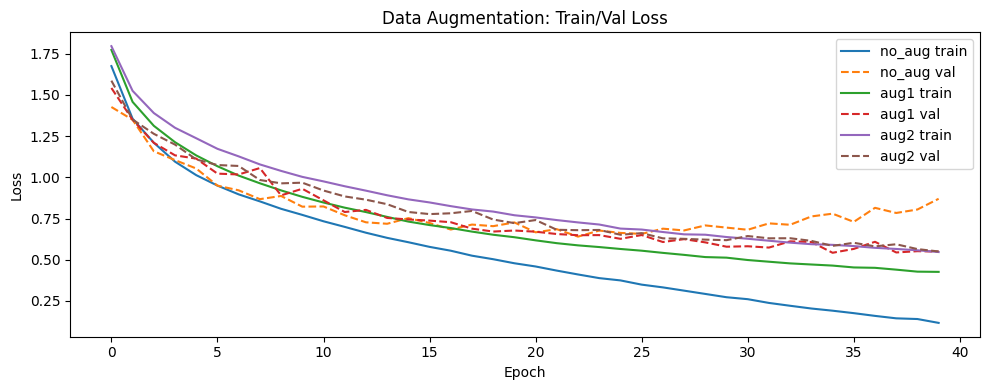
\includegraphics[width=0.9\columnwidth]{figs/net_aug_loss.png}
  \caption{Training/validation loss for no augmentation, Aug1, and Aug2.}
  \label{fig:aug_loss}
\end{figure}

\begin{itemize}
  \item \textbf{Dropout and BatchNorm.} Without augmentation, we added Dropout2d after each conv block and before the final linear layer with $p=0.3$, and BatchNorm after each convolution. These regularizers reduced validation accuracy relative to the baseline (Table~\ref{tab:net_train_acc}), suggesting underfitting at the chosen settings.
  \item \textbf{Zero initialization.} Using zeros for kernel initialization produced 10\% validation accuracy (random guess on CIFAR-10; Table~\ref{tab:net_train_acc}).
  \item \textbf{SGD learning rate sweep.} Using SGD with learning rates \{3e-3, 1e-3, 3e-4\}, the loss curves are shown in Figure~\ref{fig:sgd_loss}; higher learning rates converge faster early but show more oscillation.
\end{itemize}
\begin{figure}[!ht]
  \centering
  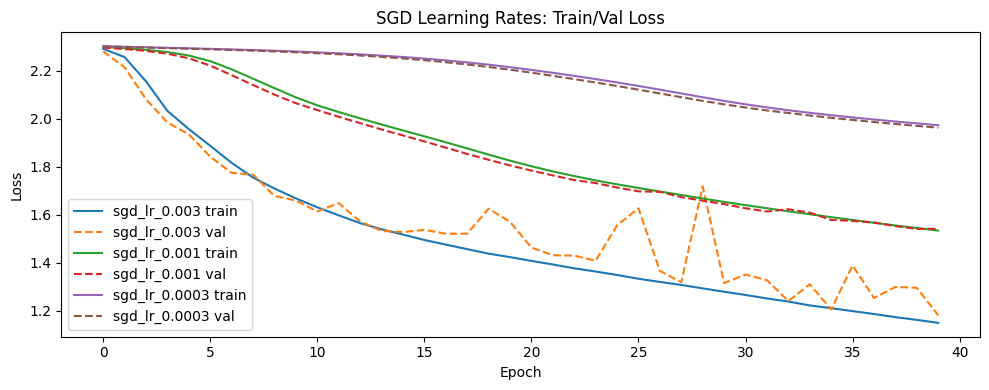
\includegraphics[width=0.9\columnwidth]{figs/net_sgd_loss.png}
  \caption{Training/validation loss for SGD learning rates 3e-3, 1e-3, and 3e-4.}
  \label{fig:sgd_loss}
\end{figure}

\begin{table}[!ht]
  \centering
  \small
  \setlength{\tabcolsep}{4pt}
  \caption{Best validation accuracy (\%) for augmentation and regularization settings.}
  \label{tab:net_train_acc}
  \begin{tabular}{lc}
    \toprule
    Setting & Best Val Acc \\
    \midrule
    aug1 & 81.71 \\
    aug2 & 81.42 \\
    no\_aug & 79.37 \\
    baseline+batchnorm+dropout & 76.83 \\
    baseline+dropout & 76.79 \\
    baseline+batchnorm & 76.02 \\
    zeros\_init & 10.00 \\
    \bottomrule
  \end{tabular}
\end{table}

